% Options for packages loaded elsewhere
% Options for packages loaded elsewhere
\PassOptionsToPackage{unicode}{hyperref}
\PassOptionsToPackage{hyphens}{url}
%
\documentclass[
  ignorenonframetext,
  aspectratio=169,
  handout]{beamer}
\newif\ifbibliography
\usepackage{pgfpages}
\setbeamertemplate{caption}[numbered]
\setbeamertemplate{caption label separator}{: }
\setbeamercolor{caption name}{fg=normal text.fg}
\beamertemplatenavigationsymbolsempty
% remove section numbering
\setbeamertemplate{part page}{
  \centering
  \begin{beamercolorbox}[sep=16pt,center]{part title}
    \usebeamerfont{part title}\insertpart\par
  \end{beamercolorbox}
}
\setbeamertemplate{section page}{
  \centering
  \begin{beamercolorbox}[sep=12pt,center]{section title}
    \usebeamerfont{section title}\insertsection\par
  \end{beamercolorbox}
}
\setbeamertemplate{subsection page}{
  \centering
  \begin{beamercolorbox}[sep=8pt,center]{subsection title}
    \usebeamerfont{subsection title}\insertsubsection\par
  \end{beamercolorbox}
}
% Prevent slide breaks in the middle of a paragraph
\widowpenalties 1 10000
\raggedbottom
\AtBeginPart{
  \frame{\partpage}
}
\AtBeginSection{
  \ifbibliography
  \else
    \frame{\sectionpage}
  \fi
}
\AtBeginSubsection{
  \frame{\subsectionpage}
}
\usepackage{iftex}
\ifPDFTeX
  \usepackage[T1]{fontenc}
  \usepackage[utf8]{inputenc}
  \usepackage{textcomp} % provide euro and other symbols
\else % if luatex or xetex
  \usepackage{unicode-math} % this also loads fontspec
  \defaultfontfeatures{Scale=MatchLowercase}
  \defaultfontfeatures[\rmfamily]{Ligatures=TeX,Scale=1}
\fi
\usepackage{lmodern}

\ifPDFTeX\else
  % xetex/luatex font selection
\fi
% Use upquote if available, for straight quotes in verbatim environments
\IfFileExists{upquote.sty}{\usepackage{upquote}}{}
\IfFileExists{microtype.sty}{% use microtype if available
  \usepackage[]{microtype}
  \UseMicrotypeSet[protrusion]{basicmath} % disable protrusion for tt fonts
}{}
\makeatletter
\@ifundefined{KOMAClassName}{% if non-KOMA class
  \IfFileExists{parskip.sty}{%
    \usepackage{parskip}
  }{% else
    \setlength{\parindent}{0pt}
    \setlength{\parskip}{6pt plus 2pt minus 1pt}}
}{% if KOMA class
  \KOMAoptions{parskip=half}}
\makeatother


\usepackage{longtable,booktabs,array}
\newcounter{none} % for unnumbered tables
\usepackage{calc} % for calculating minipage widths
\usepackage{caption}
% Make caption package work with longtable
\makeatletter
\def\fnum@table{\tablename~\thetable}
\makeatother
\usepackage{graphicx}
\makeatletter
\newsavebox\pandoc@box
\newcommand*\pandocbounded[1]{% scales image to fit in text height/width
  \sbox\pandoc@box{#1}%
  \Gscale@div\@tempa{\textheight}{\dimexpr\ht\pandoc@box+\dp\pandoc@box\relax}%
  \Gscale@div\@tempb{\linewidth}{\wd\pandoc@box}%
  \ifdim\@tempb\p@<\@tempa\p@\let\@tempa\@tempb\fi% select the smaller of both
  \ifdim\@tempa\p@<\p@\scalebox{\@tempa}{\usebox\pandoc@box}%
  \else\usebox{\pandoc@box}%
  \fi%
}
% Set default figure placement to htbp
\def\fps@figure{htbp}
\makeatother





\setlength{\emergencystretch}{3em} % prevent overfull lines

\providecommand{\tightlist}{%
  \setlength{\itemsep}{0pt}\setlength{\parskip}{0pt}}



 


\makeatletter
\@ifpackageloaded{caption}{}{\usepackage{caption}}
\AtBeginDocument{%
\ifdefined\contentsname
  \renewcommand*\contentsname{Table of contents}
\else
  \newcommand\contentsname{Table of contents}
\fi
\ifdefined\listfigurename
  \renewcommand*\listfigurename{List of Figures}
\else
  \newcommand\listfigurename{List of Figures}
\fi
\ifdefined\listtablename
  \renewcommand*\listtablename{List of Tables}
\else
  \newcommand\listtablename{List of Tables}
\fi
\ifdefined\figurename
  \renewcommand*\figurename{Figure}
\else
  \newcommand\figurename{Figure}
\fi
\ifdefined\tablename
  \renewcommand*\tablename{Table}
\else
  \newcommand\tablename{Table}
\fi
}
\@ifpackageloaded{float}{}{\usepackage{float}}
\floatstyle{ruled}
\@ifundefined{c@chapter}{\newfloat{codelisting}{h}{lop}}{\newfloat{codelisting}{h}{lop}[chapter]}
\floatname{codelisting}{Listing}
\newcommand*\listoflistings{\listof{codelisting}{List of Listings}}
\makeatother
\makeatletter
\makeatother
\makeatletter
\@ifpackageloaded{caption}{}{\usepackage{caption}}
\@ifpackageloaded{subcaption}{}{\usepackage{subcaption}}
\makeatother

\usepackage{bookmark}
\IfFileExists{xurl.sty}{\usepackage{xurl}}{} % add URL line breaks if available
\urlstyle{same}
\hypersetup{
  pdftitle={Wave-Particle Duality},
  pdfauthor={Davit Potoyan},
  hidelinks,
  pdfcreator={LaTeX via pandoc}}


\title{\texorpdfstring{Wave-Particle Duality}{Wave-Particle Duality}}
\subtitle{\texorpdfstring{Chem 3240 · Lecture
1.5}{Chem 3240 · Lecture 1.5}}
\author{Davit Potoyan}
\date{}

\begin{document}
\frame{\titlepage}


\begin{frame}
\begin{block}{The Big Idea}
\protect\phantomsection\label{the-big-idea}
\begin{itemize}
\tightlist
\item
  \textbf{Particles and waves are not mutually exclusive}
\item
  Every quantum object shows \textbf{both} behaviors
\end{itemize}

\begin{itemize}
\tightlist
\item
  An electron has a \textbf{wavelength}; a photon has \textbf{momentum}
\end{itemize}

\begin{itemize}
\tightlist
\item
  Which behavior dominates depends on the \textbf{experimental
  conditions}
\end{itemize}
\end{block}

\begin{block}{Diffraction and Interference}
\protect\phantomsection\label{diffraction-and-interference}
\begin{columns}[T]
\begin{column}{0.5\linewidth}
\includegraphics[width=0.9\linewidth,height=\textheight,keepaspectratio]{../../ch01/images/ext_double_slit.gif}
\end{column}

\begin{column}{0.5\linewidth}
\begin{itemize}
\tightlist
\item
  \textbf{Diffraction:} waves spread around obstacles or through
  openings
\item
  \textbf{Interference:} combined waves add (in phase) or cancel (out of
  phase)
\item
  \textbf{Double slit:} two slits produce interference bands on the
  screen
\end{itemize}
\end{column}
\end{columns}
\end{block}

\begin{block}{Bragg's Law: X-rays Scatter Off Crystals}
\protect\phantomsection\label{braggs-law-x-rays-scatter-off-crystals}
\begin{columns}[T]
\begin{column}{0.5\linewidth}
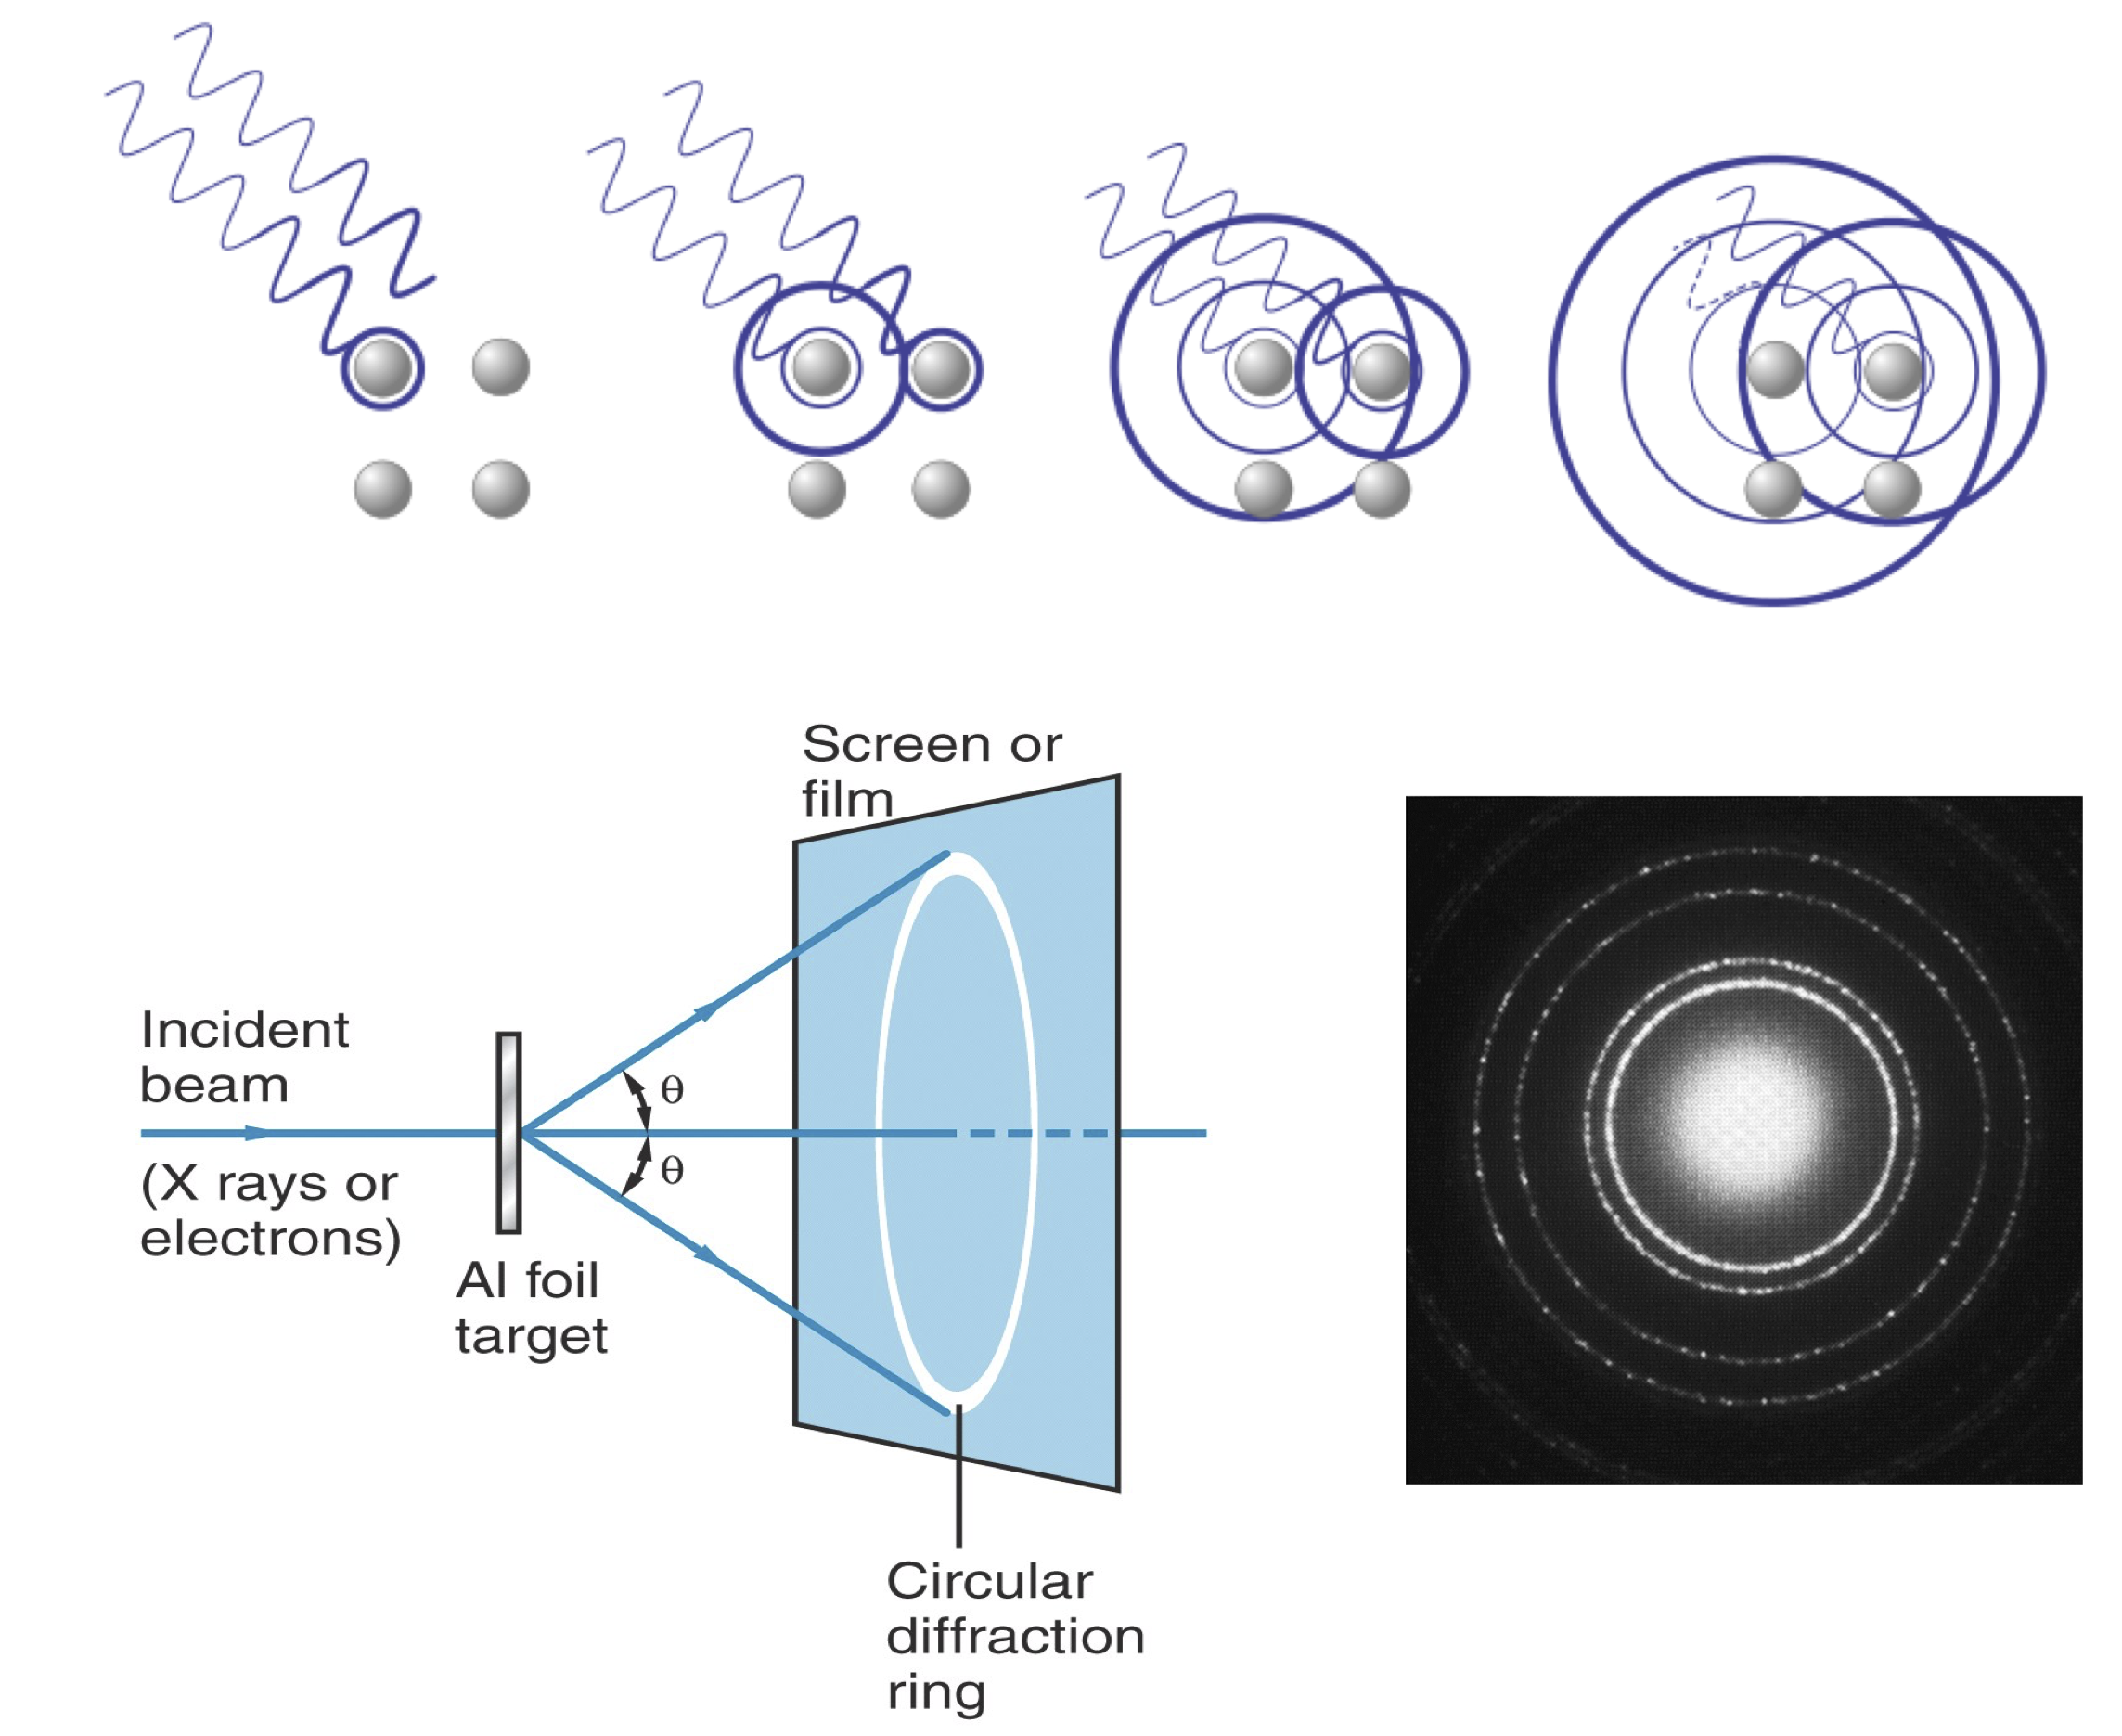
\includegraphics[width=0.9\linewidth,height=\textheight,keepaspectratio]{../../ch01/images/lec3_Xscatter2.png}
\end{column}

\begin{column}{0.5\linewidth}
\begin{itemize}
\tightlist
\item
  X-rays scatter off lattice atoms
\item
  Path differences give \textbf{constructive} (left) or
  \textbf{destructive} (right) interference
\end{itemize}
\end{column}
\end{columns}

\[\boxed{2d \sin\theta = n\lambda}\]

\begin{itemize}
\tightlist
\item
  \(d\): plane spacing, \(\lambda\): wavelength, \(n\): diffraction
  order
\item
  Interference was the \textbf{hallmark of wave behavior}
\end{itemize}
\end{block}

\begin{block}{Electrons Also Diffract}
\protect\phantomsection\label{electrons-also-diffract}
\begin{columns}[T]
\begin{column}{0.5\linewidth}
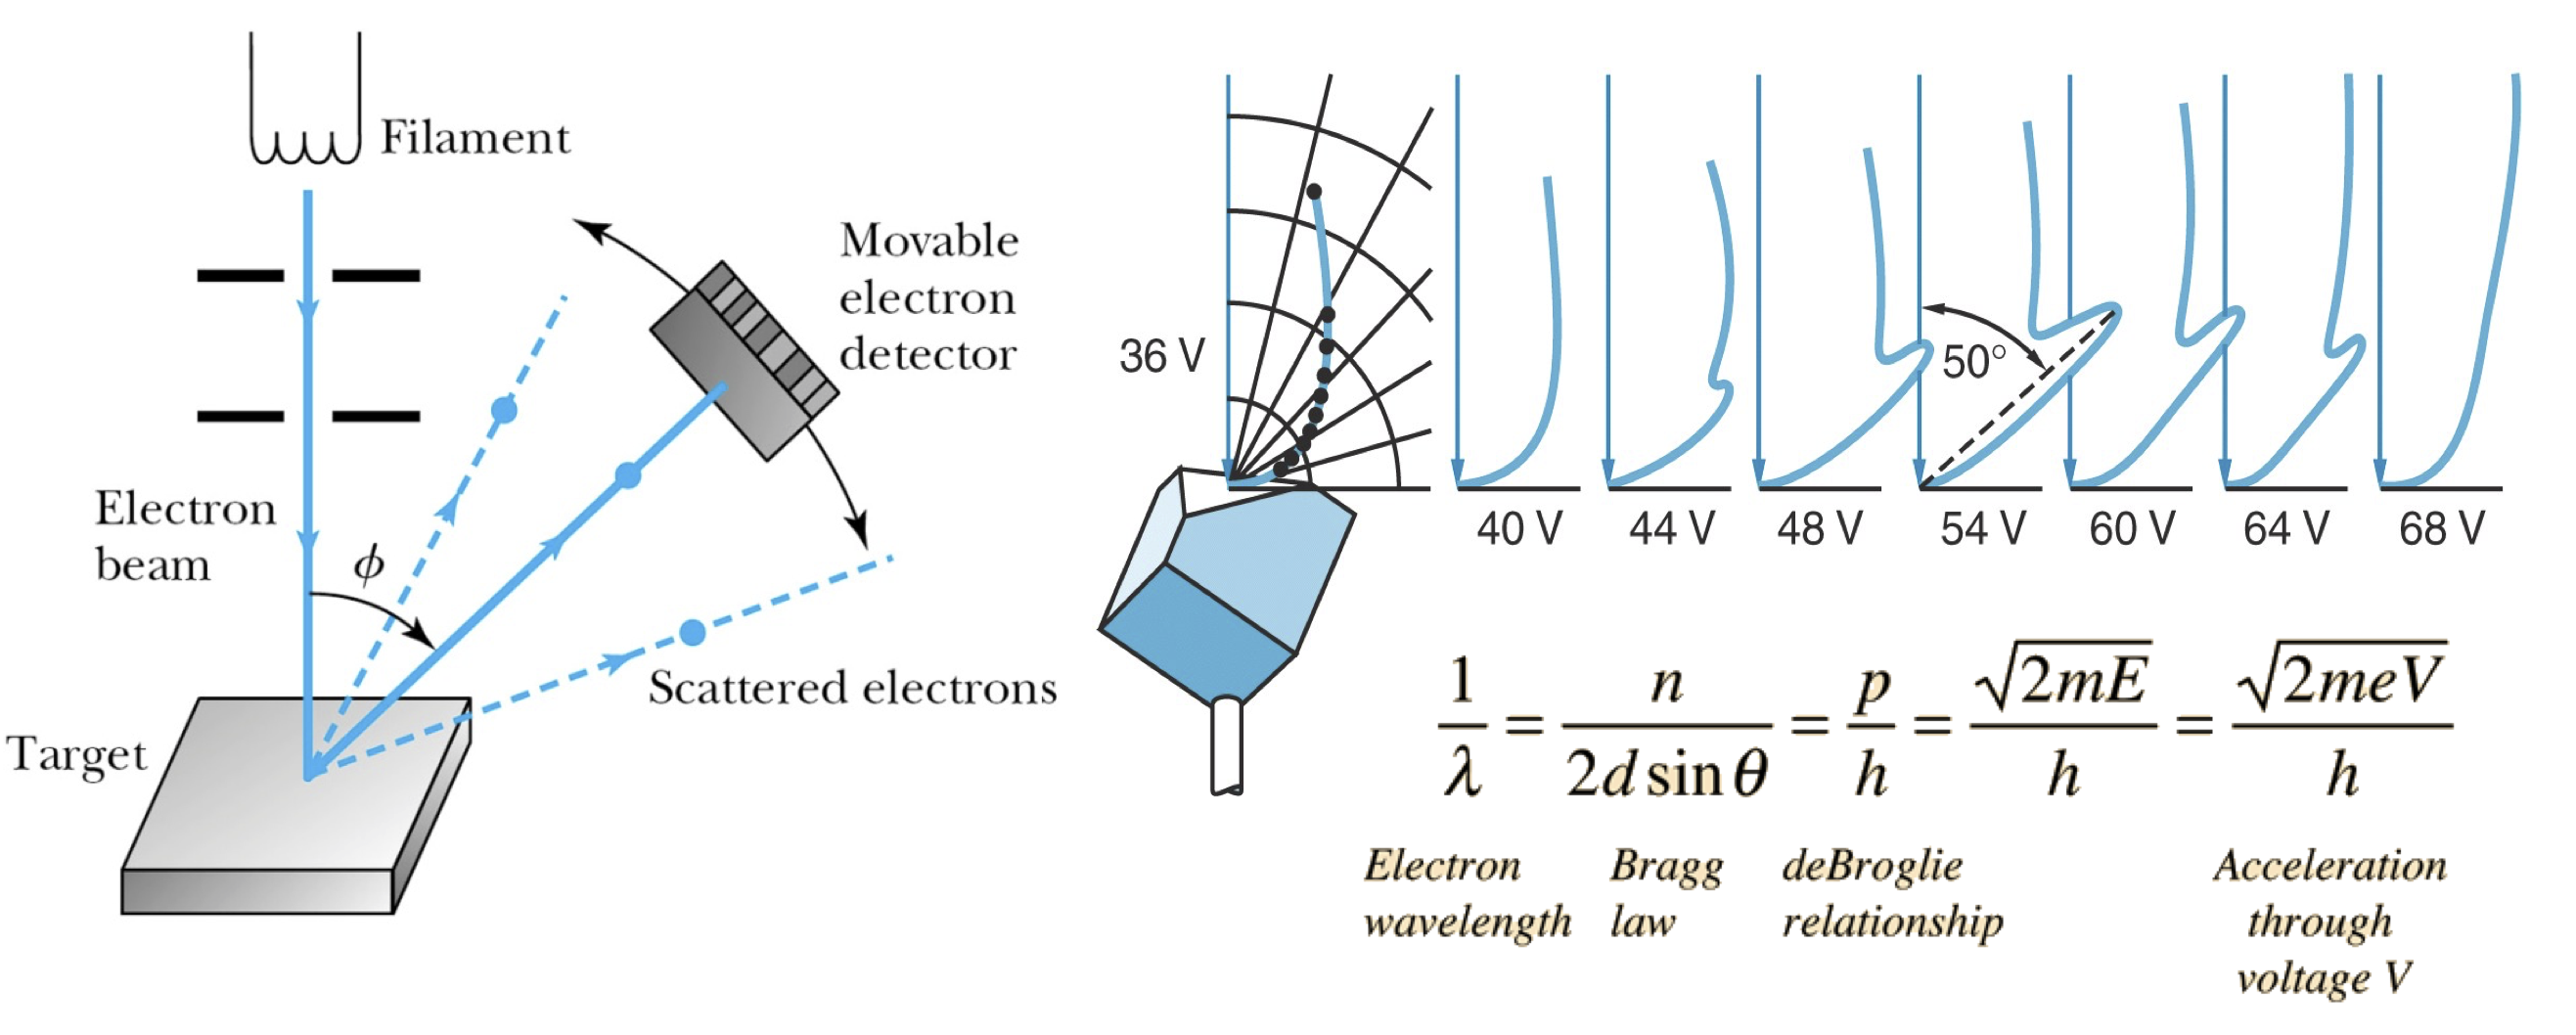
\includegraphics[width=0.95\linewidth,height=\textheight,keepaspectratio]{../../ch01/images/lec3_DavisonGermer.png}
\end{column}

\begin{column}{0.5\linewidth}
\begin{itemize}
\tightlist
\item
  \textbf{Davisson and Germer (1925):} intensity peaks in scattered
  electron beams
\item
  Peaks fit \textbf{Bragg's law} (until then only for X-rays)
\item
  Electrons behave as \textbf{waves}
\end{itemize}
\end{column}
\end{columns}
\end{block}

\begin{block}{Compton Scattering: Light Has Momentum}
\protect\phantomsection\label{compton-scattering-light-has-momentum}
\begin{columns}[T]
\begin{column}{0.5\linewidth}
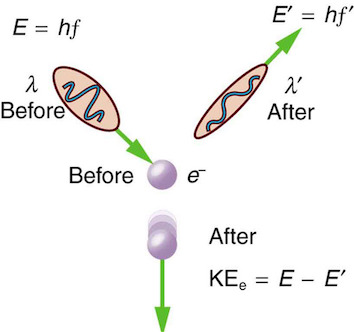
\includegraphics[width=0.9\linewidth,height=\textheight,keepaspectratio]{../../ch01/images/lec3_compton.jpeg}
\end{column}

\begin{column}{0.5\linewidth}
\begin{itemize}
\tightlist
\item
  X-rays scatter off free electrons like \textbf{billiard balls}
\item
  Conservation of \textbf{momentum} gives longer outgoing wavelength
\item
  Makes sense only if the photon is a \textbf{particle} with momentum
\end{itemize}
\end{column}
\end{columns}
\end{block}

\begin{block}{The de Broglie Relation}
\protect\phantomsection\label{the-de-broglie-relation}
\begin{itemize}
\tightlist
\item
  Wave-like and particle-like traits are \textbf{inversely proportional}
\end{itemize}

\[\boxed{\lambda = \frac{h}{p}}\]

\begin{itemize}
\tightlist
\item
  \(h\): Planck's constant, \(p\): momentum, \(\lambda\): wavelength
\item
  \textbf{Heavy/fast} objects: tiny wavelength (particle-like)
\item
  \textbf{Light/slow} objects: large wavelength (wave-like)
\end{itemize}

\begin{itemize}
\tightlist
\item
  With \(E = T + V\): \(\quad \lambda = \dfrac{h}{\sqrt{2m(E - V)}}\)
\item
  Wavelength \textbf{changes} as a particle moves through different
  potentials (key for bonding)
\end{itemize}
\end{block}

\begin{block}{The Double-Slit Puzzle}
\protect\phantomsection\label{the-double-slit-puzzle}
\begin{columns}[T]
\begin{column}{0.5\linewidth}
\includegraphics[width=0.9\linewidth,height=\textheight,keepaspectratio]{../../ch01/images/ext_wave_particle_duality.gif}
\end{column}

\begin{column}{0.5\linewidth}
\begin{itemize}
\tightlist
\item
  Electrons build an \textbf{interference pattern}
\item
  It persists even with \textbf{one electron at a time}
\item
  Each electron interferes with \textbf{itself}
\end{itemize}
\end{column}
\end{columns}
\end{block}

\begin{block}{Which Slit?}
\protect\phantomsection\label{which-slit}
\begin{columns}[T]
\begin{column}{0.5\linewidth}
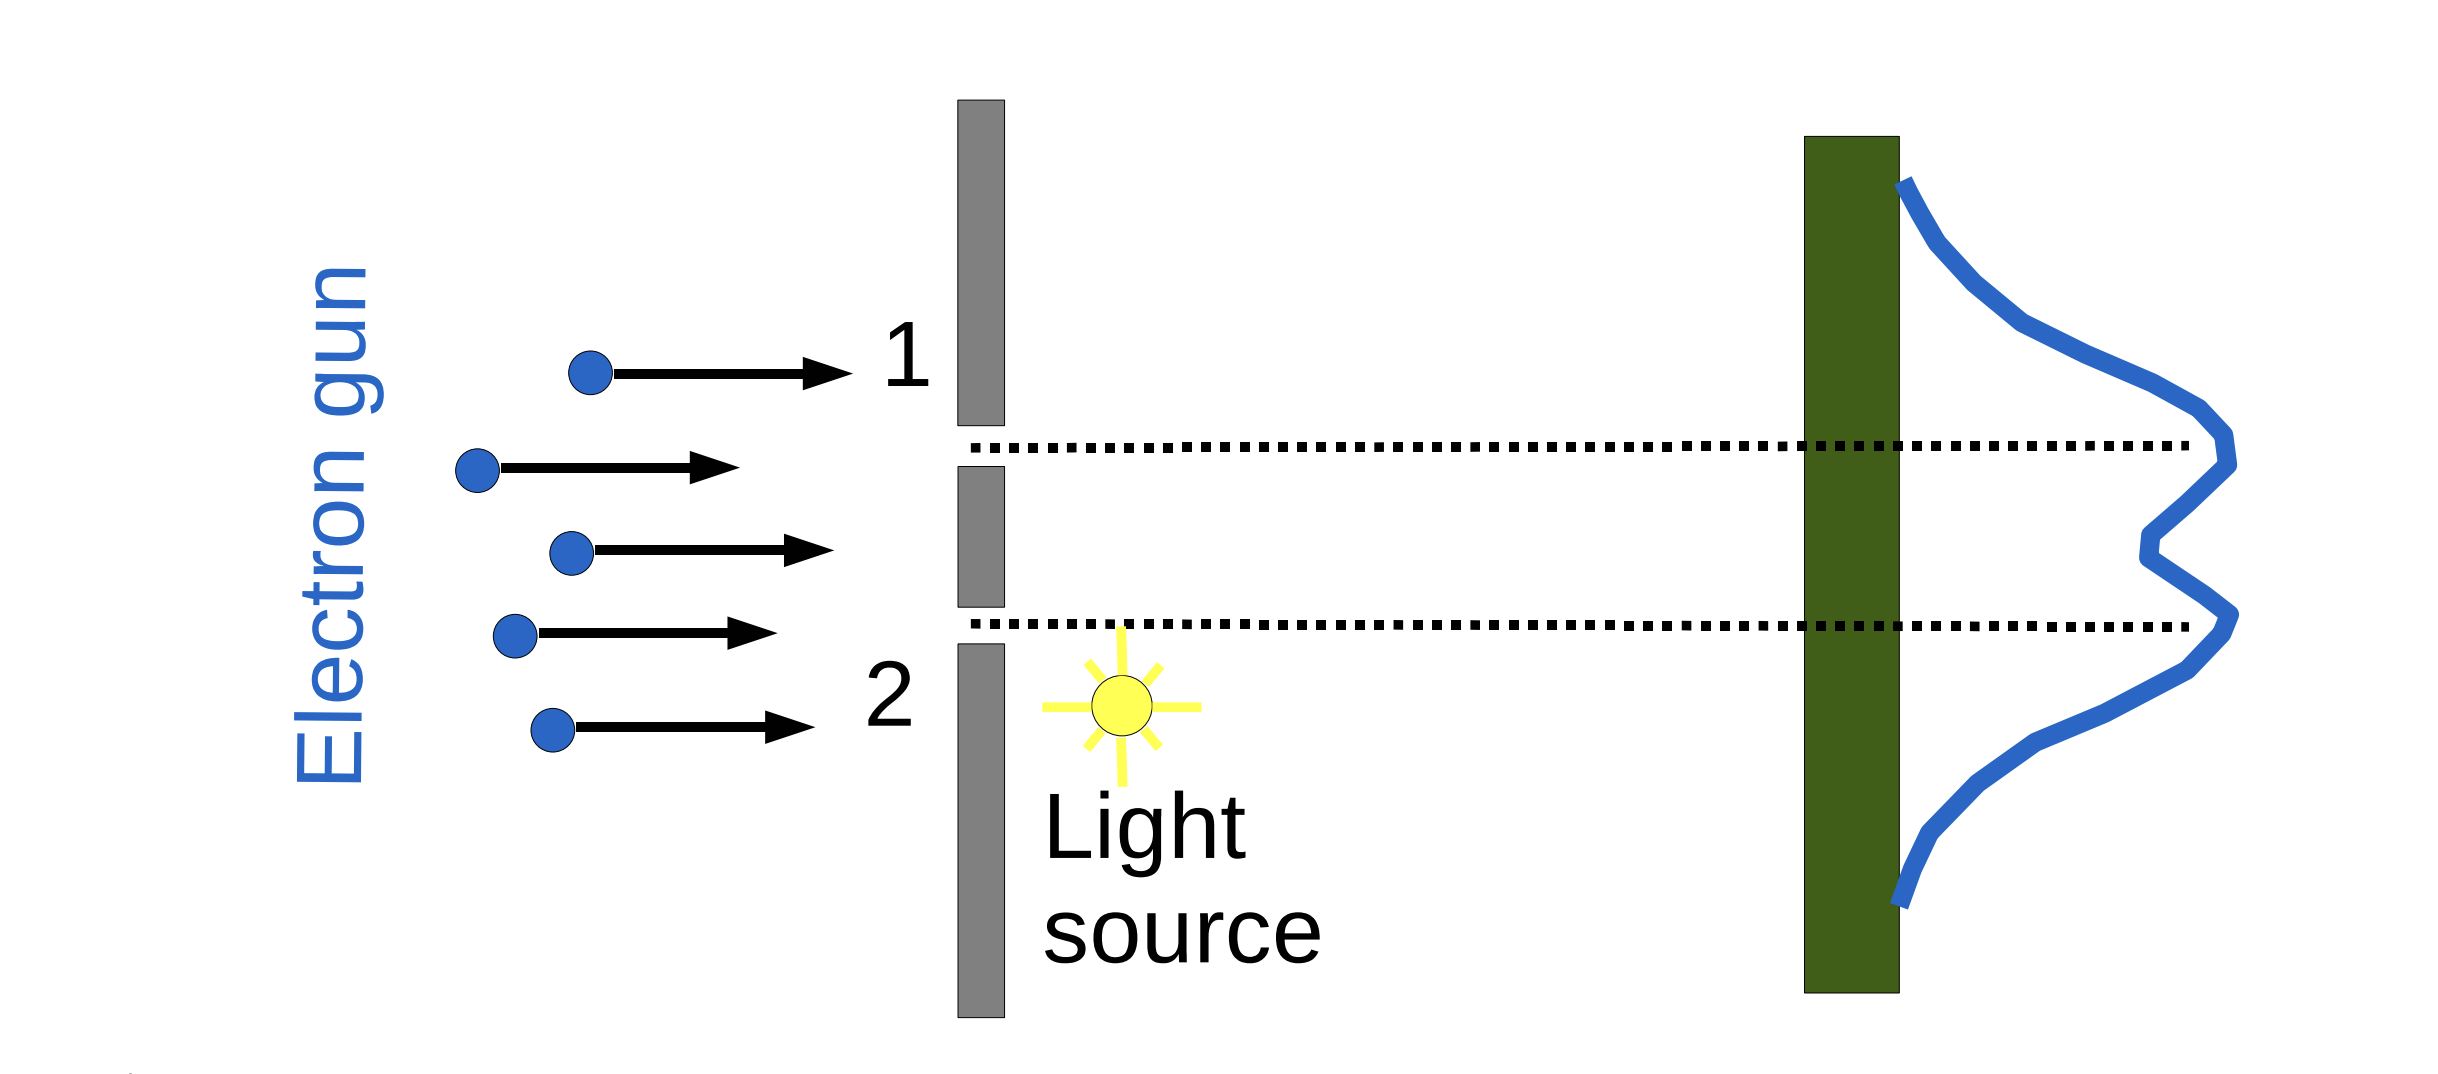
\includegraphics[width=0.9\linewidth,height=\textheight,keepaspectratio]{../../ch01/images/double_slit2.png}
\end{column}

\begin{column}{0.5\linewidth}
\begin{itemize}
\tightlist
\item
  Try to detect \textbf{which slit} the electron took
\item
  The \textbf{interference pattern disappears}
\item
  Measurement changes the outcome (resolved later via QM postulates)
\end{itemize}
\end{column}
\end{columns}
\end{block}

\begin{block}{Heisenberg's Uncertainty Principle}
\protect\phantomsection\label{heisenbergs-uncertainty-principle}
\begin{columns}[T]
\begin{column}{0.5\linewidth}
\includegraphics[width=0.9\linewidth,height=\textheight,keepaspectratio]{../../ch01/images/ext_uncertainty_momentum.gif}
\end{column}

\begin{column}{0.5\linewidth}
\begin{itemize}
\tightlist
\item
  Cannot know exact \textbf{position and momentum} at once
\item
  Narrow the slit (localize \(x\)): momentum spreads out
\item
  A direct consequence of \textbf{wave-particle duality}
\end{itemize}
\end{column}
\end{columns}

\[\sigma_x \sigma_p \geq \hbar/2\]
\end{block}
\end{frame}

\begin{frame}{Takeaway}
\protect\phantomsection\label{takeaway}
\begin{quote}
Every quantum object is both wave and particle, with wavelength set by
\(\lambda = h/p\), so position and momentum can never both be sharp:
\(\sigma_x \sigma_p \geq \hbar/2\).
\end{quote}
\end{frame}




\end{document}
